\section{Results}
\label{sec:kernel_results}

We present degree and kernel mixing estimates from three different types of aggregate relational data (asking how many people do you know in subpopulation $\scriptG_k$) gathered from the same survey:
\begin{enumerate}
\item responses to questions where $\mathcal{G}_k$ are 12 names
\item responses to questions where $\mathcal{G}_k$ are 8 occupations
\item both sets of responses from (1) and (2)
\end{enumerate}

% Names Results
\subsection{Names}
\label{sec:kernel_results_names}

We first let $\mathcal{G}_k$ be equal to the 12 subpopulations with the following names
\begin{itemize}
\item Linda ($\mu_1 = 63.3, \sigma_1 = 10.5$)
\item Jennifer ($\mu_1 = 37.4, \sigma_1 = 10.6$)
\item Karen ($\mu_1 = 56.1, \sigma_1 = 14.0$)
\item Kimberly ($\mu_1 = 39.8, \sigma_1 = 13.0$)
\item Emily ($\mu_1 = 28.4, \sigma_1 = 23.4$)
\item Stephanie ($\mu_1 = 35.6, \sigma_1 = 14.4$)
\item Mark ($\mu_2 = 49.3, \sigma_2 = 15.1$)
\item Jacob ($\mu_2 = 22.7, \sigma_2 = 18.5$)
\item Kevin ($\mu_2 = 38.8, \sigma_2 = 16.2$)
\item Kyle ($\mu_2 = 25.6, \sigma_2 = 10.8$)
\item Adam ($\mu_2 = 31.2, \sigma_2 = 16.6$)
\item Bruce ($\mu_2 = 62.5, \sigma_2 = 16.8$).
\end{itemize}
where the $\mu_{kg_j}$ and $\sigma_{kg_j}^2$ are defined in Equation \ref{eq:subpopulation_normal_approx}. As per the guidelines provided by \citet{McCormick+others:2010}, we choose names that are prevalent across a broad range of ages so that we can minimize barrier effects. Since each of the above subpopulations are specific to either males or females, however, only one value of $g_j$ is defined for each subpopulation $\scriptG_k$. Consequently, in the negative binomial expectation of Equation \ref{eq:nonrandom_mixing_kernel_with_spline}, the first summation is taken over only one value of $g_j$ for each subpopulation $\scriptG_k$.

% Names Results: Degree
\begin{figure}
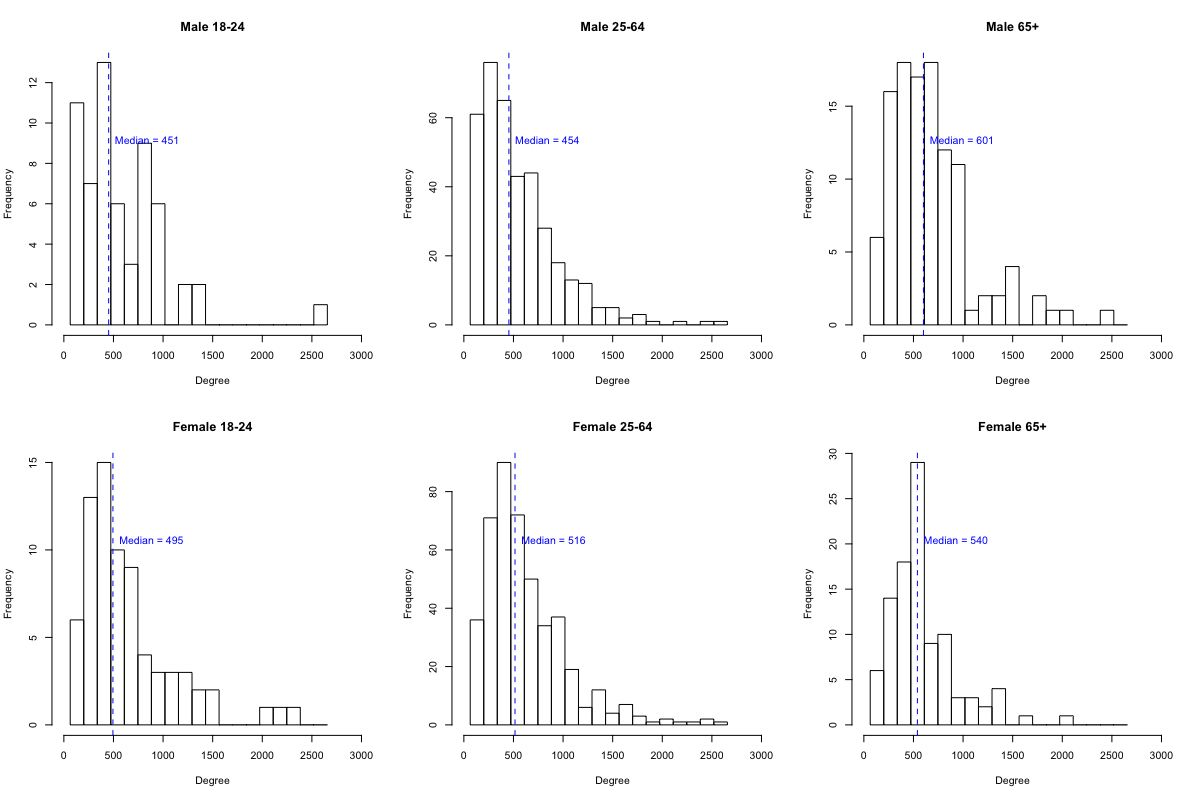
\includegraphics[width=\textwidth]{figures/kernel/names/deg_sexage.png}
\caption{Name-based degree estimates for both genders across three age groups. A pattern of degree increasing with age is clear.}
\label{fig:names_degree_sexage}
\end{figure}

Figure \ref{fig:names_degree_sexage} displays the degree estimates obtained from fitting the kernel mixing model to the names responses, for six different age-sex groups. The pattern of degree increasing with age is surprising because we usually expect degree to decrease for older individuals. However, this may partially be explained by a combination of people retiring at increasingly older ages and in general being more active at older ages than in the past.

% Names Results: Kernel
\begin{figure}
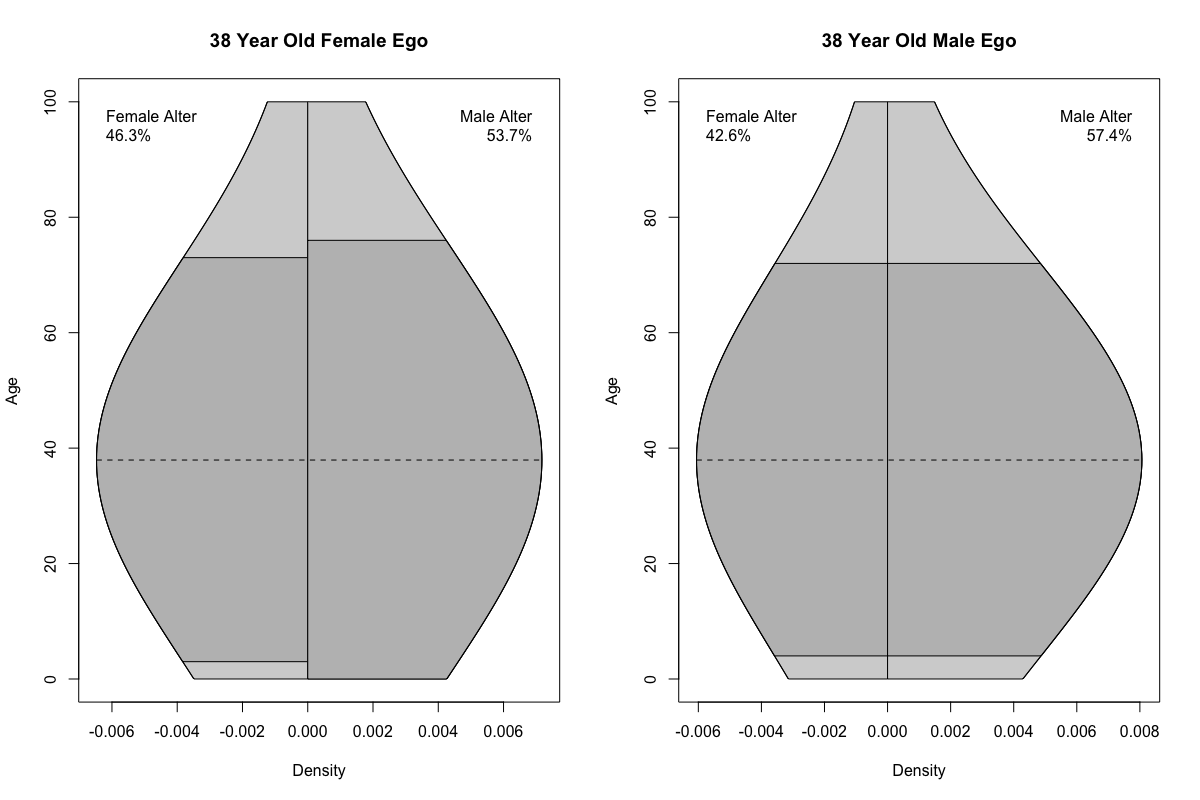
\includegraphics[width=0.9\textwidth]{figures/kernel/names/kern_sexage.png}
\caption{Name-based kernel estimates for male and female egos of age 21, 38, and 70. The darker regions show one standard deviation of the kernel.}
\label{fig:names_kernel_sexage}
\end{figure}

Figure \ref{fig:names_kernel_sexage} displays the kernel estimates for male and female egos of three different ages, each. Compared to the mixing matrix in Figure \ref{fig:nonrandom_mixing_matrix}, the kernels show more regularity in their structure from ego to ego (by design). Additionally, estimating kernel bandwidth as a function of age allows us to clearly see how the age concentration of alters changes by age. Meanwhile, the gender mixing matrix, while simpler than the age-gender mixing matrix, is still able to capture the variability in network composition by gender. In particular, it appears that female egos' social networks are roughly equally split between males (51.1\%) and females (49.9\%), but male egos' social networks contain more males (55.5\%) than females (44.5\%).

% Names Results: Kernel Bandwidth Spline
\begin{figure}
\centering
	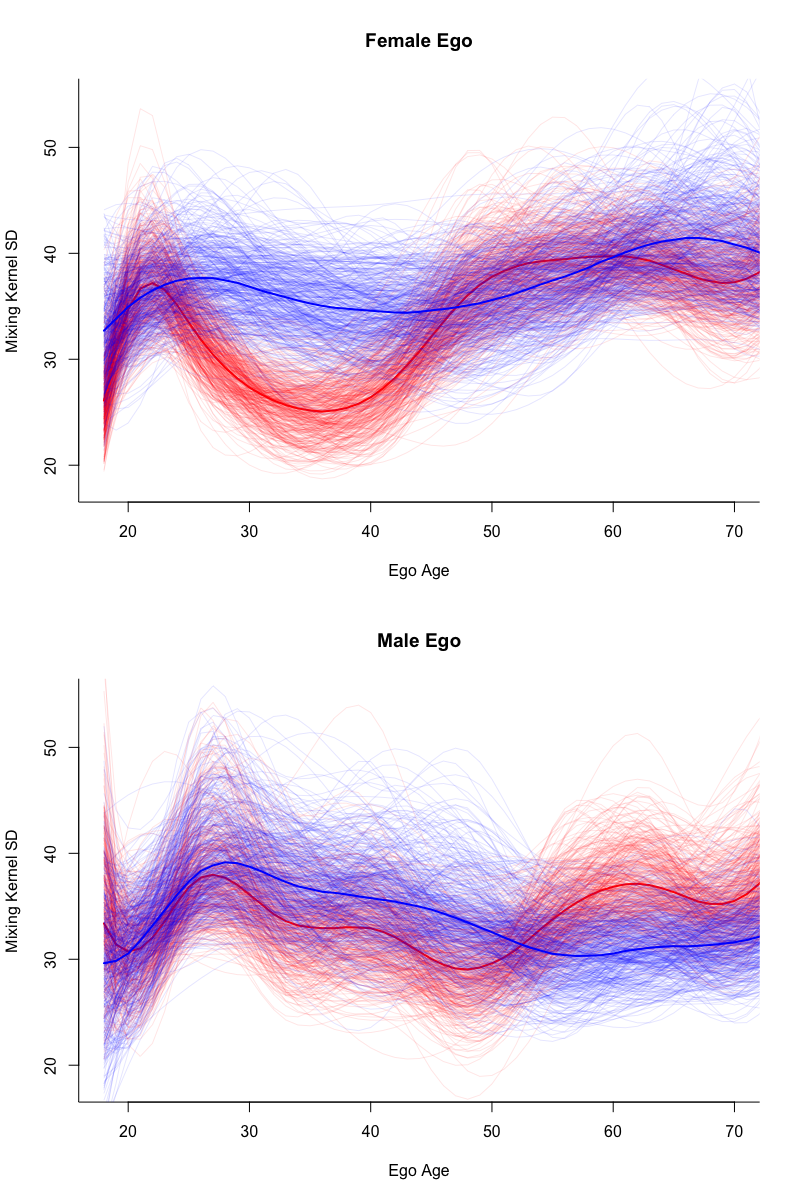
\includegraphics[width=0.7\textwidth]{figures/kernel/names/kern_spline_overlay.png}
\caption{Posterior draws of name-based kernel bandwidth splines for male and female egos. Blue draws correspond to male alters while red draws correspond to female alters. Individual draws are shown with 0.1 alpha while medians are shown with 1.0 alpha.}
\label{fig:names_kernel_spline}
\end{figure}

Figure \ref{fig:names_kernel_spline} displays the kernel bandwidth spline estimates by ego and alter gender. Male egos' social network age distributions are more spread out (i.e. larger bandwidth) when they first enter the work force in their late 20s, and then the networks' age distributions gradually tighten as the egos get older. Female egos' social network age distributions, on the other hand, spread out slightly earlier on, and sharply decrease going into the 30s, perhaps due to childbirth. However, after age 40, their networks' age distributions spread out again, stabilizing in the 60s.

% Occupations Results
\subsection{Occupations}
\label{sec:kernel_results_occs}

We next let $\mathcal{G}_k$ be equal to the 8 subpopulations with the following occupations
\begin{itemize}
\item Professor ($\mu_1 = 47.8, \sigma_1 = 15.0;  \mu_2 = 48.8, \sigma_2 = 16.3$)
\item Childcare Worker ($\mu_1 = 40.0, \sigma_1 = 15.3; \mu_2 = 34.0, \sigma_2 = 18.2$)
\item Police Officer ($\mu_1 = 39.5, \sigma_1 = 9.2; \mu_2 = 40.6, \sigma_2 = 10.9$)
\item Lawyer ($\mu_1 = 48.0, \sigma_1 = 11.3; \mu_2 = 51.2, \sigma_2 = 13.3$)
\item Social Worker ($\mu_1 = 45.3, \sigma_1 = 12.9; \mu_2 = 45.0, \sigma_2 = 13.8$)
\item Electrician ($\mu_1 = 45.7, \sigma_1 = 13.4; \mu_2 = 43.1, \sigma_2 = 12.5$)
\item Cosmetologist ($\mu_1 =  42.4, \sigma_1 = 14.9; \mu_2 = 45.6, \sigma_2 = 19.5$)
\item Bartender ($\mu_1 = 37.9, \sigma_1 = 13.6; \mu_2 = 38.2, \sigma_2 = 13.1$).
\end{itemize}
Unlike the names in the previous section, there are two genders of subpopulations for each occupation. As such, $\mu_{kg_j}$ and $\sigma_{kg_j}$ are defined for both values of $g_j$, and the first summation of Equation \ref{eq:nonrandom_mixing_kernel_with_spline} is taken over both values of $g_j$. 

% Occupation Results: Degree
\begin{figure}
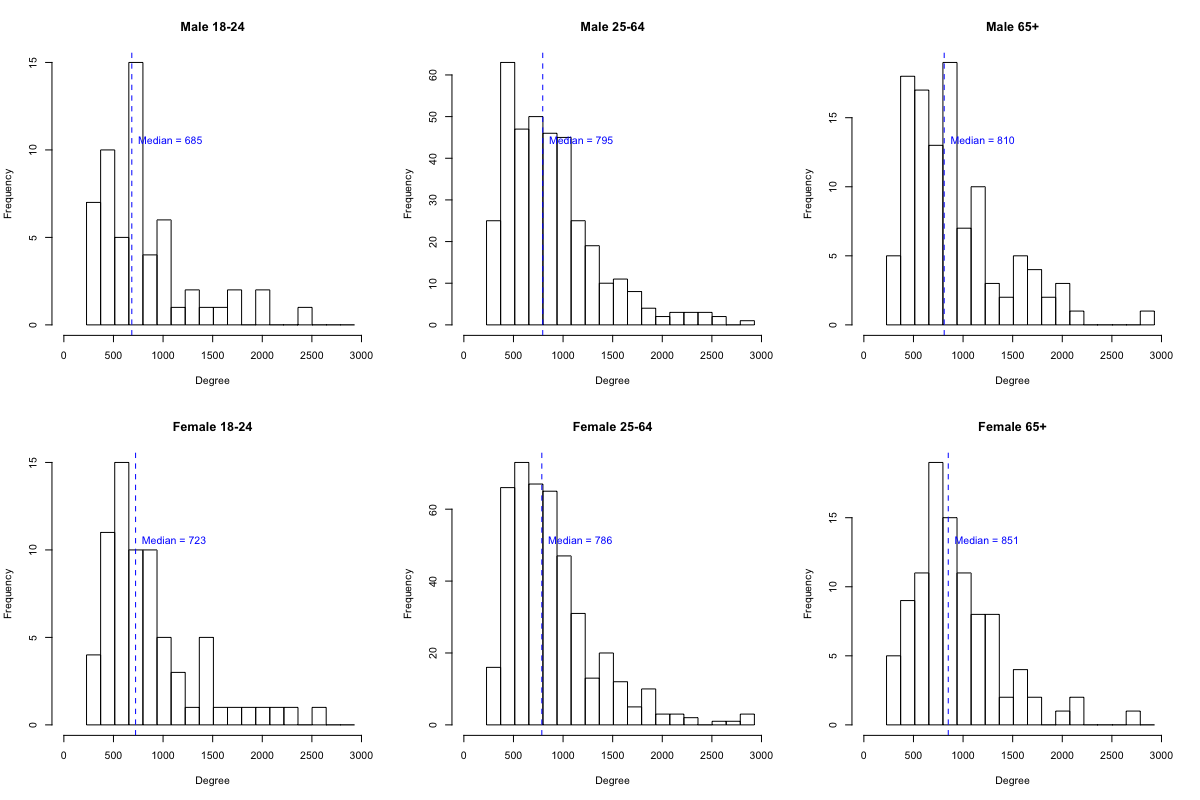
\includegraphics[width=\textwidth]{figures/kernel/occs/deg_sexage.png}
\caption{Occupation-based degree estimates for both genders across three age groups. }
\label{fig:occs_degree_sexage}
\end{figure}

Figure \ref{fig:occs_degree_sexage} displays the degree estimates obtained from fitting the kernel mixing model to the occupations responses, for six different age-sex groups. As with the names, here we see a pattern of degree increasing with age. However, the the degree estimates themselves are in the 700-850 range, compared to the 450-600 range for the names-based estimates. This is likely due to the fact that the population occupation data is only available for individuals 18 and older. As a result, the normalizing constant in Equation \ref{eq:nonrandom_mixing_kernel_with_spline}
\begin{align}
C_{kg_j} = \sum_a \frac{N_{k,a, g_j}}{N_{a,g_j}} \label{eq:kernel_normalizing_constant}
\end{align}
is smaller than it is for names, which are observed in the population for all ages, including under 18 years old. Since the summation $C_{kg_j}$ is multiplicative with respect to ego degree $d_i$ in the negative binomial expectation of Equation \ref{eq:nonrandom_mixing_kernel_with_spline}, a decrease in the summation's value causes an increase in the degree estimates when all other terms in the expectation are held constant. This suggests that occupations (and subpopulations $\scriptG_k$ that are age restricted in general) should not be used if one's goal is to obtain accurate degree estimates.

% Occupation Results: Kernel
\begin{figure}
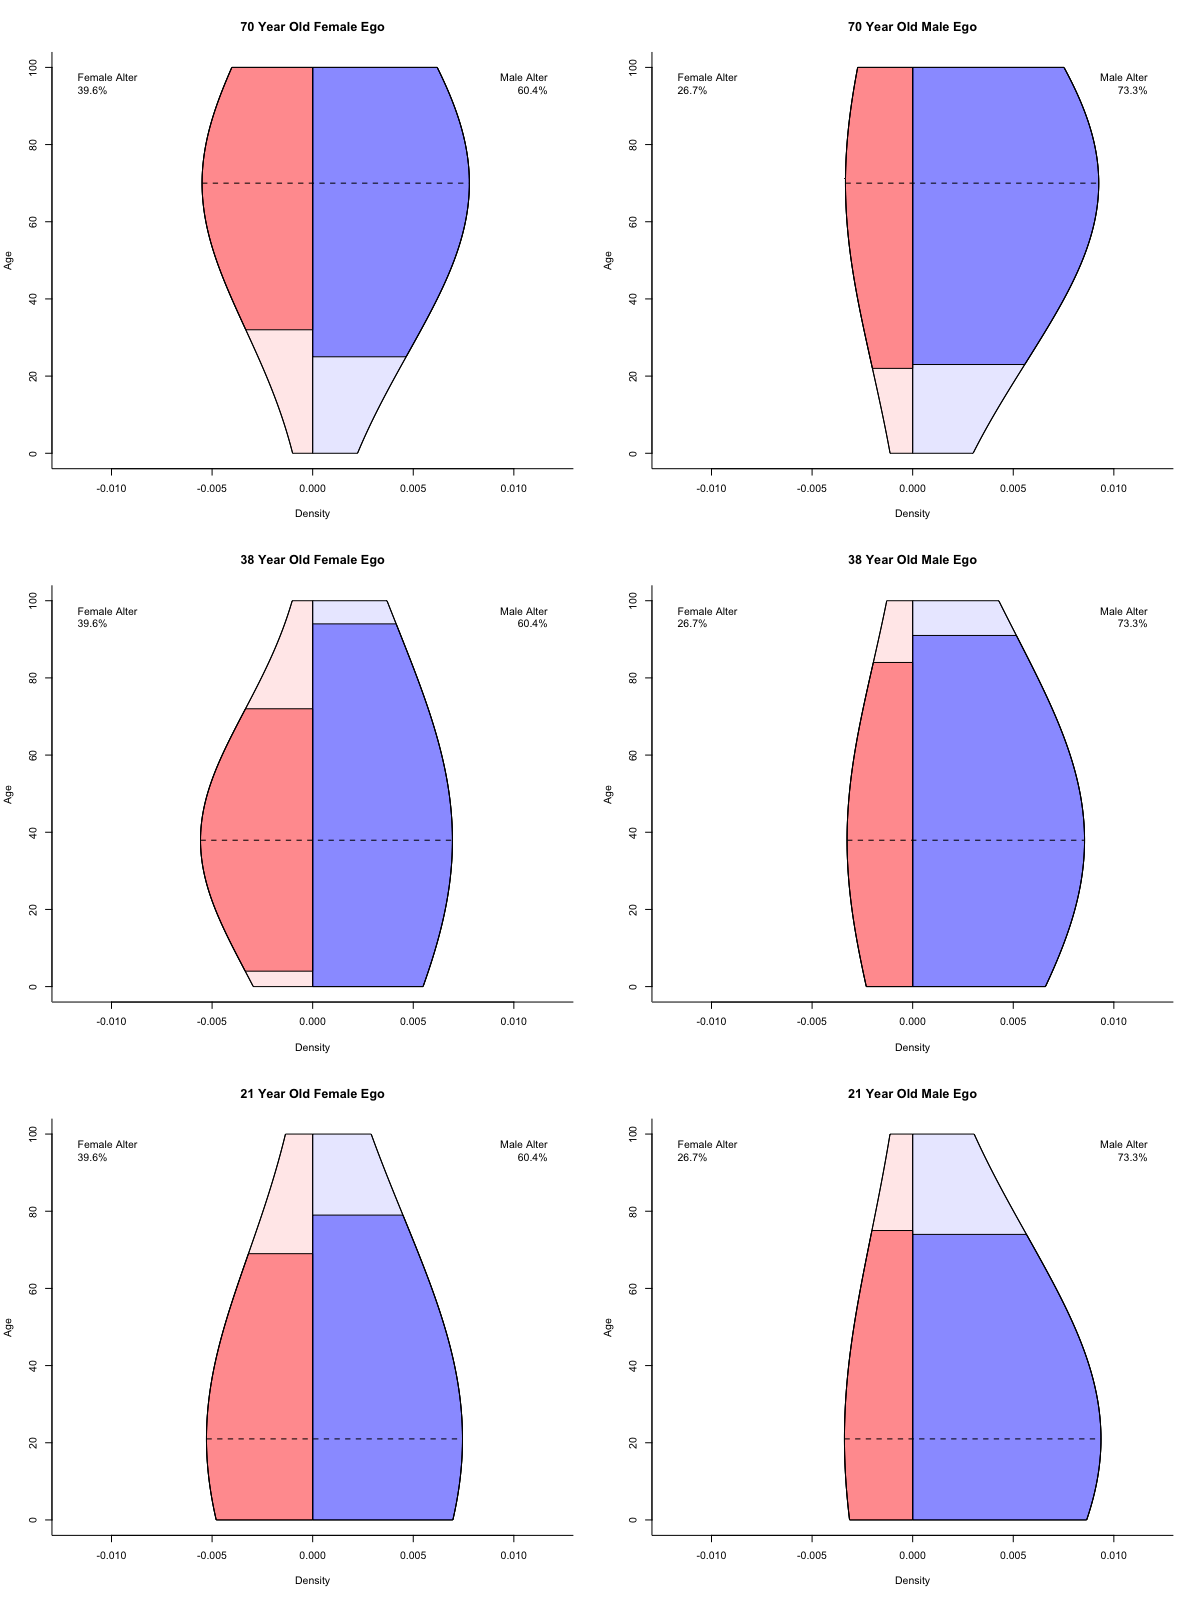
\includegraphics[width=0.9\textwidth]{figures/kernel/occs/kern_sexage.png}
\caption{Occupation-based kernel estimates for male and female egos of age 21, 38, and 70. The darker regions show one standard deviation of the kernel.}
\label{fig:occs_kernel_sexage}
\end{figure}

Figure \ref{fig:occs_kernel_sexage} displays the kernel estimates for male and female egos of three different ages, each. Compared to the name-based kernels in Figure \ref{fig:names_kernel_sexage}, the occupation-based kernels are more heavily male skewed for male and female alters. In particular, female egos' social networks are estimated to be composed of 60.4\% males and 39.6\% females, while male egos' social networks are estimated to be composed of 73.3\% males and 26.7\% females. 

Given that our surveys include more female-dominated occupations (Childcare Worker, Social Worker, and Cosmetologist) than male-dominated occupations (Police and Electrician), this skew in the kernels has a few possible explanations. From a mathematical perspective, with respect to the negative binomial expectation in Equation \ref{eq:nonrandom_mixing_kernel_with_spline}, the consequence is that for each individual, the occurrence of larger normalizing summations $C_{kg_j}$ for female-dominated occupations in the likelihood causes a decrease in the value of $\rho_{g_ig_j}$ for female alters (since an individual's degree $d_i$ is fixed for all $\rho_{g_ig_j}$ and $C_{kg_j}$). 

From the perspective of transmission errors, it may be the case that men disclose their occupations more often than women do, which would cause underreporting in the survey responses, particularly to questions about female-dominated occupations. Alternatively, it may also be the case that people with certain occupations disclose their occupations to others at a relatively lower rate (perhaps due to stigma or political reasons), and that in our case those lower-disclosing occupations happen to be female-dominated.

While it is difficult to determine which of the above issues is contributing most to the skewness, we suggest that when including survey questions about subpopulations that contain both males and females (e.g. occupation, alma mater, company), one choose subpopulations $\scriptG_k$ that have roughly the same value of the normalizing summation $C_{kg_j}$ for both genders. Such subpopulations will contribute to the likelihood in a more balanced way, and will be less likely to suffer from transmission effects correlated with gender.

% Occupation Results: Kernel Bandwidth Spline
\begin{figure}
\centering
	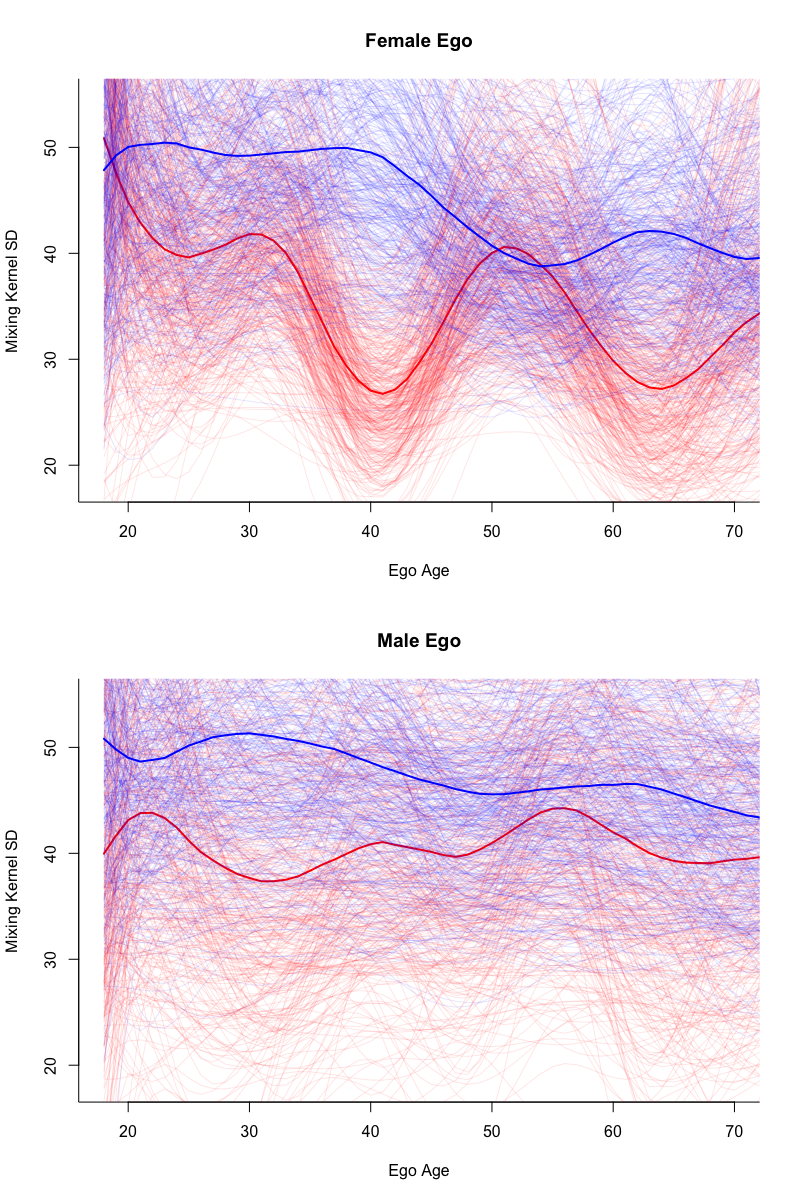
\includegraphics[width=0.7\textwidth]{figures/kernel/occs/kern_spline_overlay.png}
\caption{Posterior draws of occupation-based kernel bandwidth splines for male and female egos. Blue draws correspond to male alters while red draws correspond to female alters. Individual draws are shown with 0.1 alpha while medians are shown with 1.0 alpha}
\label{fig:occs_kernel_spline}
\end{figure}

Figure \ref{fig:occs_kernel_spline} displays the kernel bandwidth spline estimates by ego and alter gender. While the male ego splines share similar shapes to those estimated using names, the female ego splines look quite different. The splines also all show a stronger overall negative trend than the names-based estimates. Most saliently, however, the posterior variance of the splines themselves is much larger than that of the names-based estimates. This is because the expected number known $\mu_{ik}$ appears in the likelihood only 8 times (due to the 8 occupations) for each individual, whereas in the names-based approach the $\mu_{ik}$ appeared 12 times. As a result, the effective sample size is smaller, and the spline estimates are noisier. 

% Combined Results
\subsection{Combined}
\label{sec:kernel_results_comb}

We finally let $\mathcal{G}_k$ take on all of the names and occupations that were used in Sections \ref{sec:kernel_results_names} and \ref{sec:kernel_results_occs}. Thus, each survey respondent appears 20 times in the likelihood, once for a response to each of the 12 names and once for a response to each of the 8 occupations. 

% Occupation Results: Degree
\begin{figure}
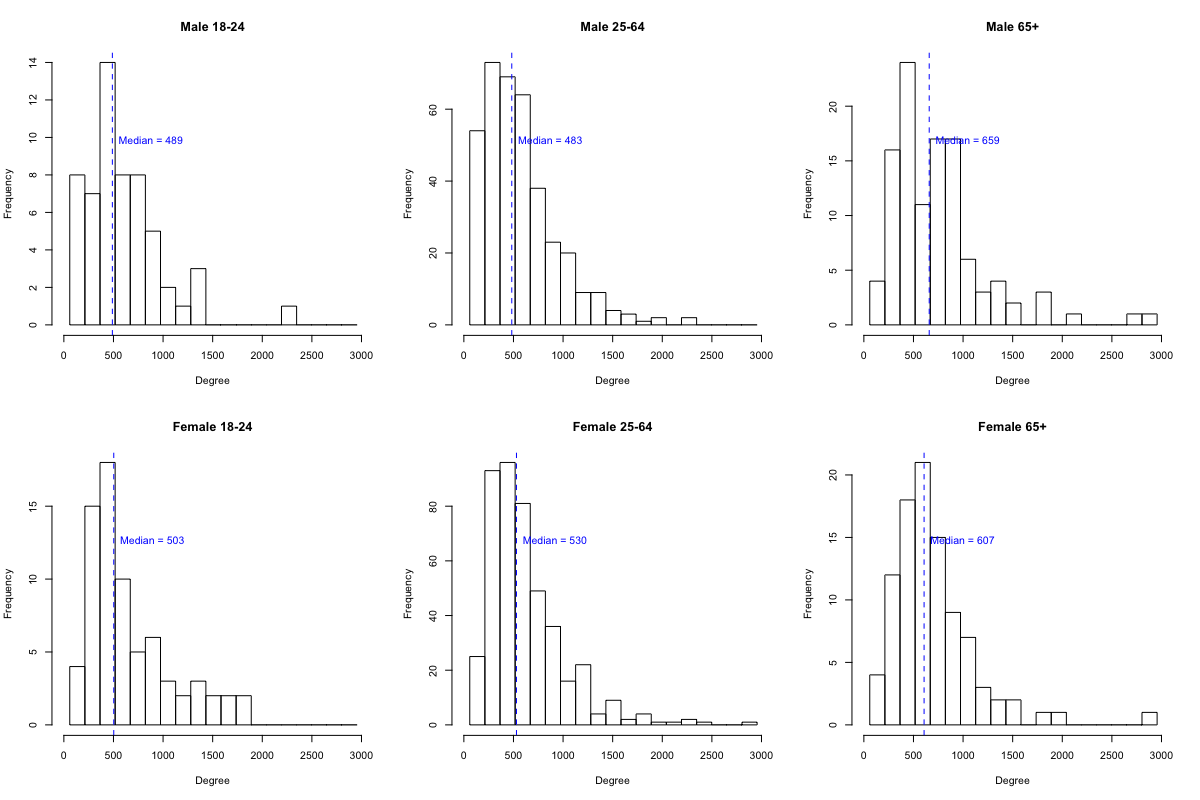
\includegraphics[width=\textwidth]{figures/kernel/comb/deg_sexage.png}
\caption{Name and occupation based degree estimates for both genders across three age groups. }
\label{fig:comb_degree_sexage}
\end{figure}

Figure \ref{fig:comb_degree_sexage} displays the degree estimates obtained from fitting the kernel mixing model to both names and occupations responses. The relative trends between the age groups are similar to the names-based estimates in Figure \ref{fig:names_degree_sexage} and the occupations-based estimates in Figure \ref{fig:occs_degree_sexage}. However, these degree estimates are in the 500-700 range, lying in between the names-only and occupations-only estimates' ranges. This middle ground is expected as the names and occupations responses both appear with $d_i$ in the likelihood. Additionally, because the names responses appear 50\% more often (there are 12 names and 8 occupations), the degree estimates are more similar to those obtained by the names-based approach in Section \ref{sec:kernel_results_names}.

% Occupation Results: Kernel
\begin{figure}
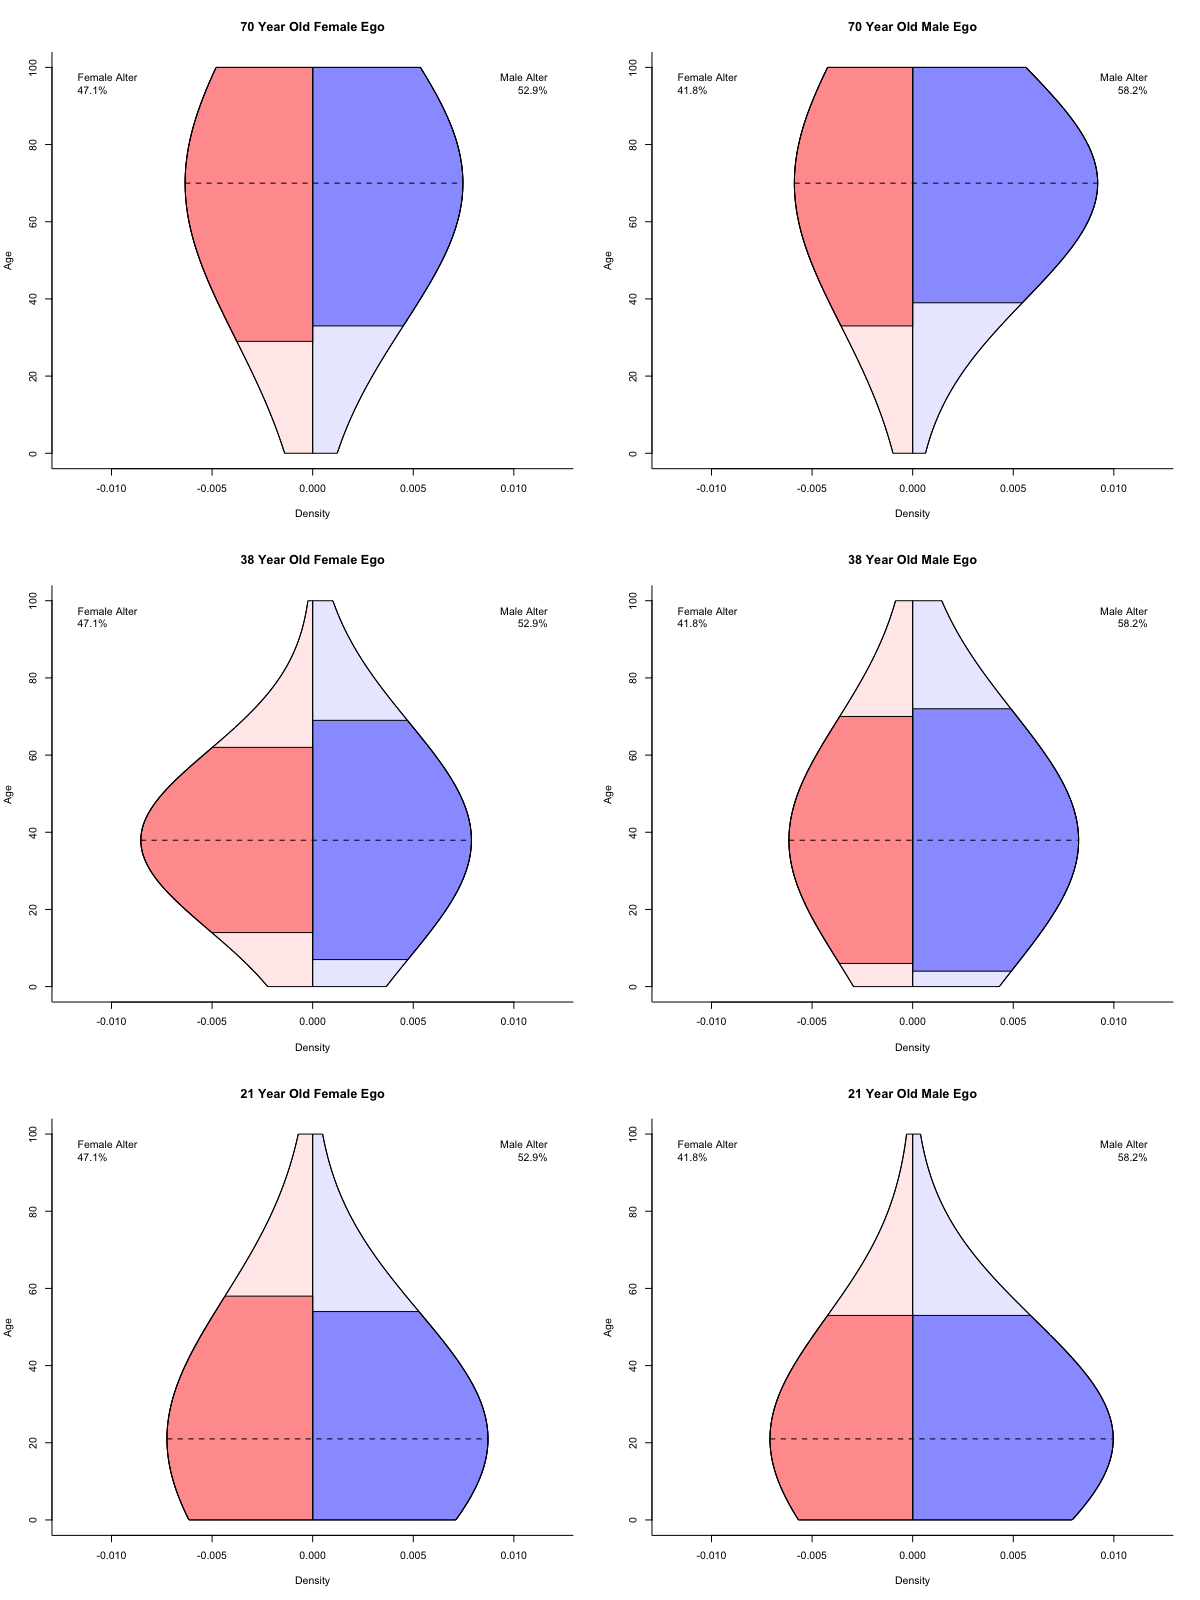
\includegraphics[width=0.9\textwidth]{figures/kernel/comb/kern_sexage.png}
\caption{Name and occupation based kernel estimates for male and female egos of age 21, 38, and 70. The darker regions show one standard deviation of the kernel.}
\label{fig:comb_kernel_sexage}
\end{figure}

Figure \ref{fig:comb_kernel_sexage} displays the kernel estimates for male and female egos of three different ages, each. The gender mixing rates are in between those estimated by the names-based approach in Section \ref{sec:kernel_results_names} and those estimated by the occupations-based approach in Section \ref{sec:kernel_results_occs}. Namely, female egos' social networks are estimated to be composed of 52.9\% males and 47.1\% females, while male egos' social networks are estimated to be composed of 58.2\% males and 41.8\% females. Overall, these proportions are more similar to the names-based estimates because there are more names than occupations in the likelihood. While these estimates seem more consistent with reality than the occupations estimates, it is not clear if this combined approach is preferable to simply using responses to names alone.

% Occupation Results: Kernel Bandwidth Spline
\begin{figure}
\centering
	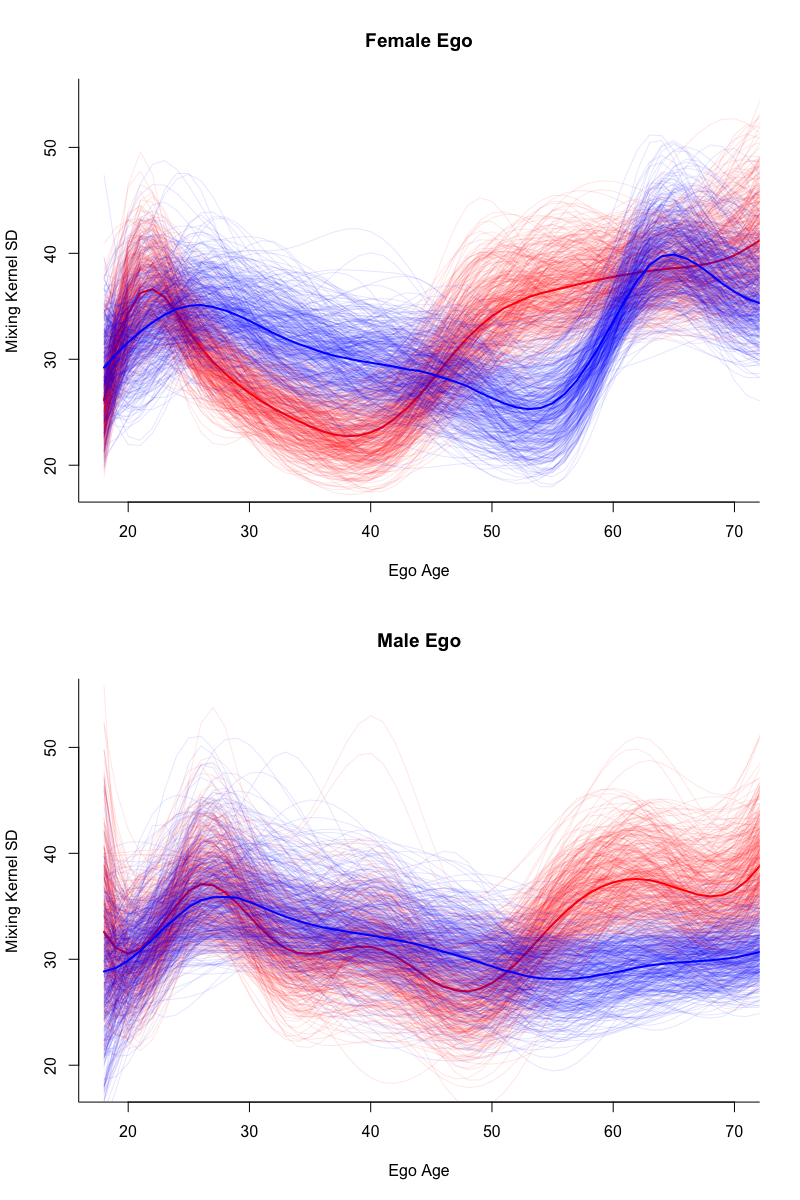
\includegraphics[width=0.7\textwidth]{figures/kernel/comb/kern_spline_overlay.png}
\caption{Posterior draws of name-and-occupation-based kernel bandwidth splines for male and female egos. Blue draws correspond to male alters while red draws correspond to female alters. Individual draws are shown with 0.1 alpha while medians are shown with 1.0 alpha}
\label{fig:comb_kernel_spline}
\end{figure}

Figure \ref{fig:comb_kernel_spline} displays the kernel bandwidth spline estimates by ego and alter gender. The overall shapes of the splines are quite similar to those estimated by the names-based approach in Figure \ref{fig:names_kernel_spline}, though the increase in the bandwidth for older female egos is more pronounced here. Furthermore, the posterior variance of the splines is smaller due to the fact that occupations responses are also included in the likelihood. 